\section{Initial Investigation}  \label{sec:initInvest}
On initial investigation of the data, one finds that the Mariana trench is represented by three matrices. The matrices represent the depth (size $1320 \times 1440$), longitude (size $1320 \times 1$), and latitude (size $1440 \times 1$) of the data recorded. In the future we will refer to the depth matrix as $\matr{A}$. Plots of the data can be seen in \autoref{fig:intialMarianaMesh}
\begin{figure}[H]
    \centering
    \subfloat[\centering 3D Plot of $\mtrA$]
    {{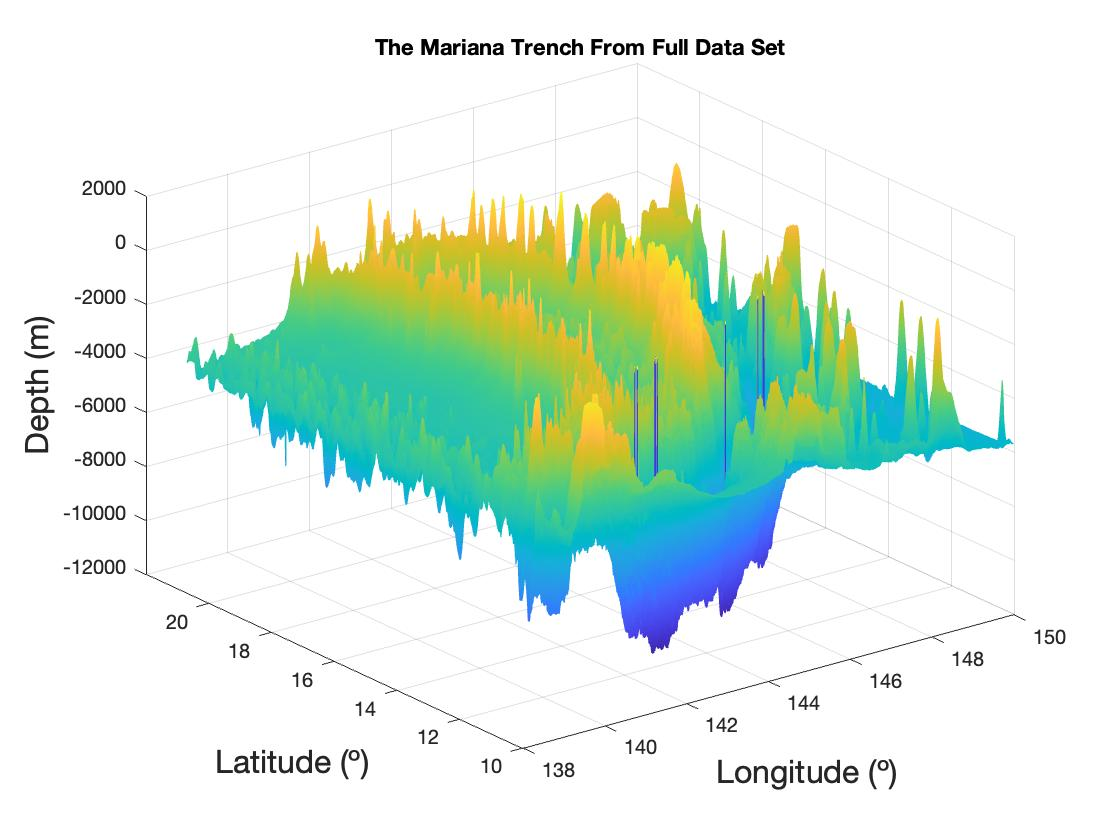
\includegraphics[width=0.45\textwidth]{./imgs/trueDataRendering.jpg}}}%
    \qquad
    \subfloat[\centering 2D Plot of $\mtrA$]
    {{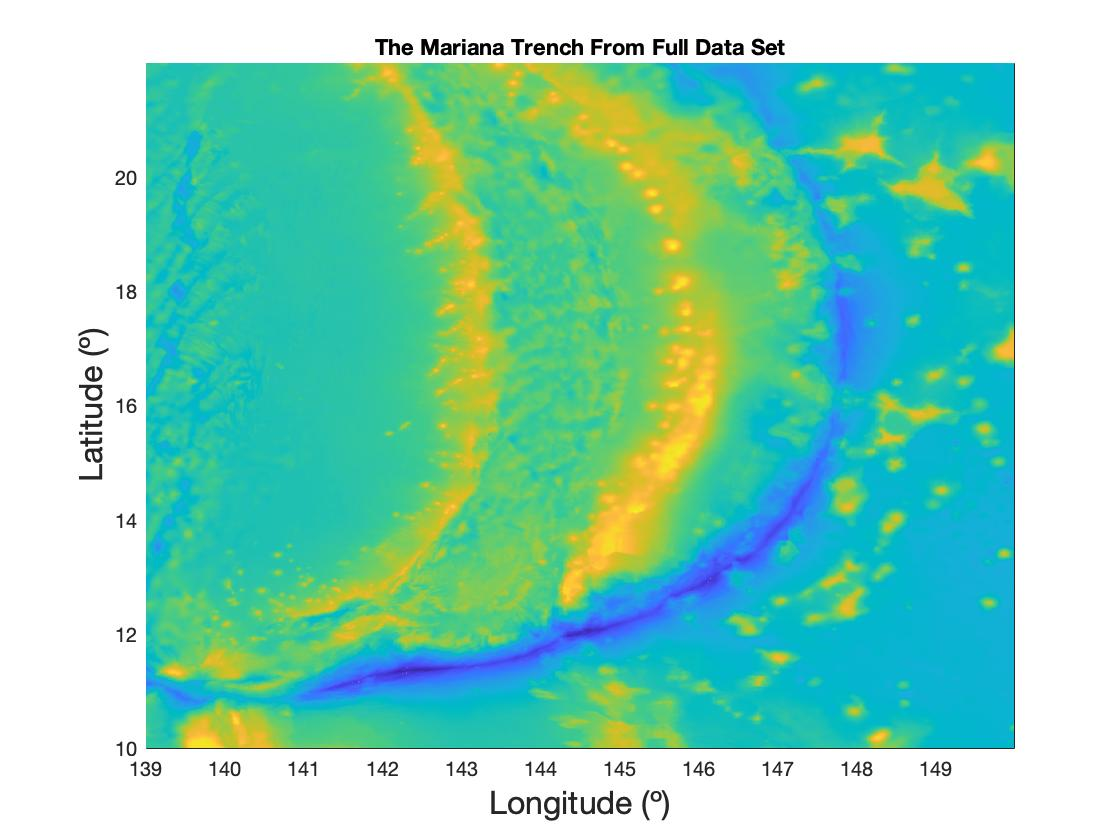
\includegraphics[width=0.45\textwidth]{./imgs/twoDFullDataSet.jpg}}}%
    \caption{Plots of Mariana Trench Depth, $\matr{A}$, in terms of latitude and longitude}%
    \label{fig:intialMarianaMesh}%
\end{figure}
Exploring this data, we find that the deepest point in the trench is $10.93$ km below sea level at a latitude of $11.333\degree$ and a  longitude of $142.2\degree$. See Section \ref{sec:codeWithOutput} for the code used. In addition, nominally defining the ocean floor to have a depth of $6$ kilometers, we can find the average depth of the trench by finding the mean of the values below 6 kilometers in $\matr{A}$. Thus, we find the average depth of the Mariana Trench to be $7.205$ km. See Section \ref{sec:codeWithOutput} for the computation used.
